\chapter{Inhalt der CD}

\begin{itemize}
	\item Master-Thesis
	\item Simulationsmodelle
		\subitem IAF.slx
		\subitem config.m für den IAF
		\subitem B6\_Buck.slx
		\subitem config.m für den B6 Buck
	
	\item Halbleitermodelle
\end{itemize}

\chapter{Anhang}

\setcounter{figure}{0}
\renewcommand{\thefigure}{A\arabic{figure}}

\setcounter{table}{0}
\renewcommand{\thetable}{A\arabic{table}}

\begin{figure}[H]
	\centering
	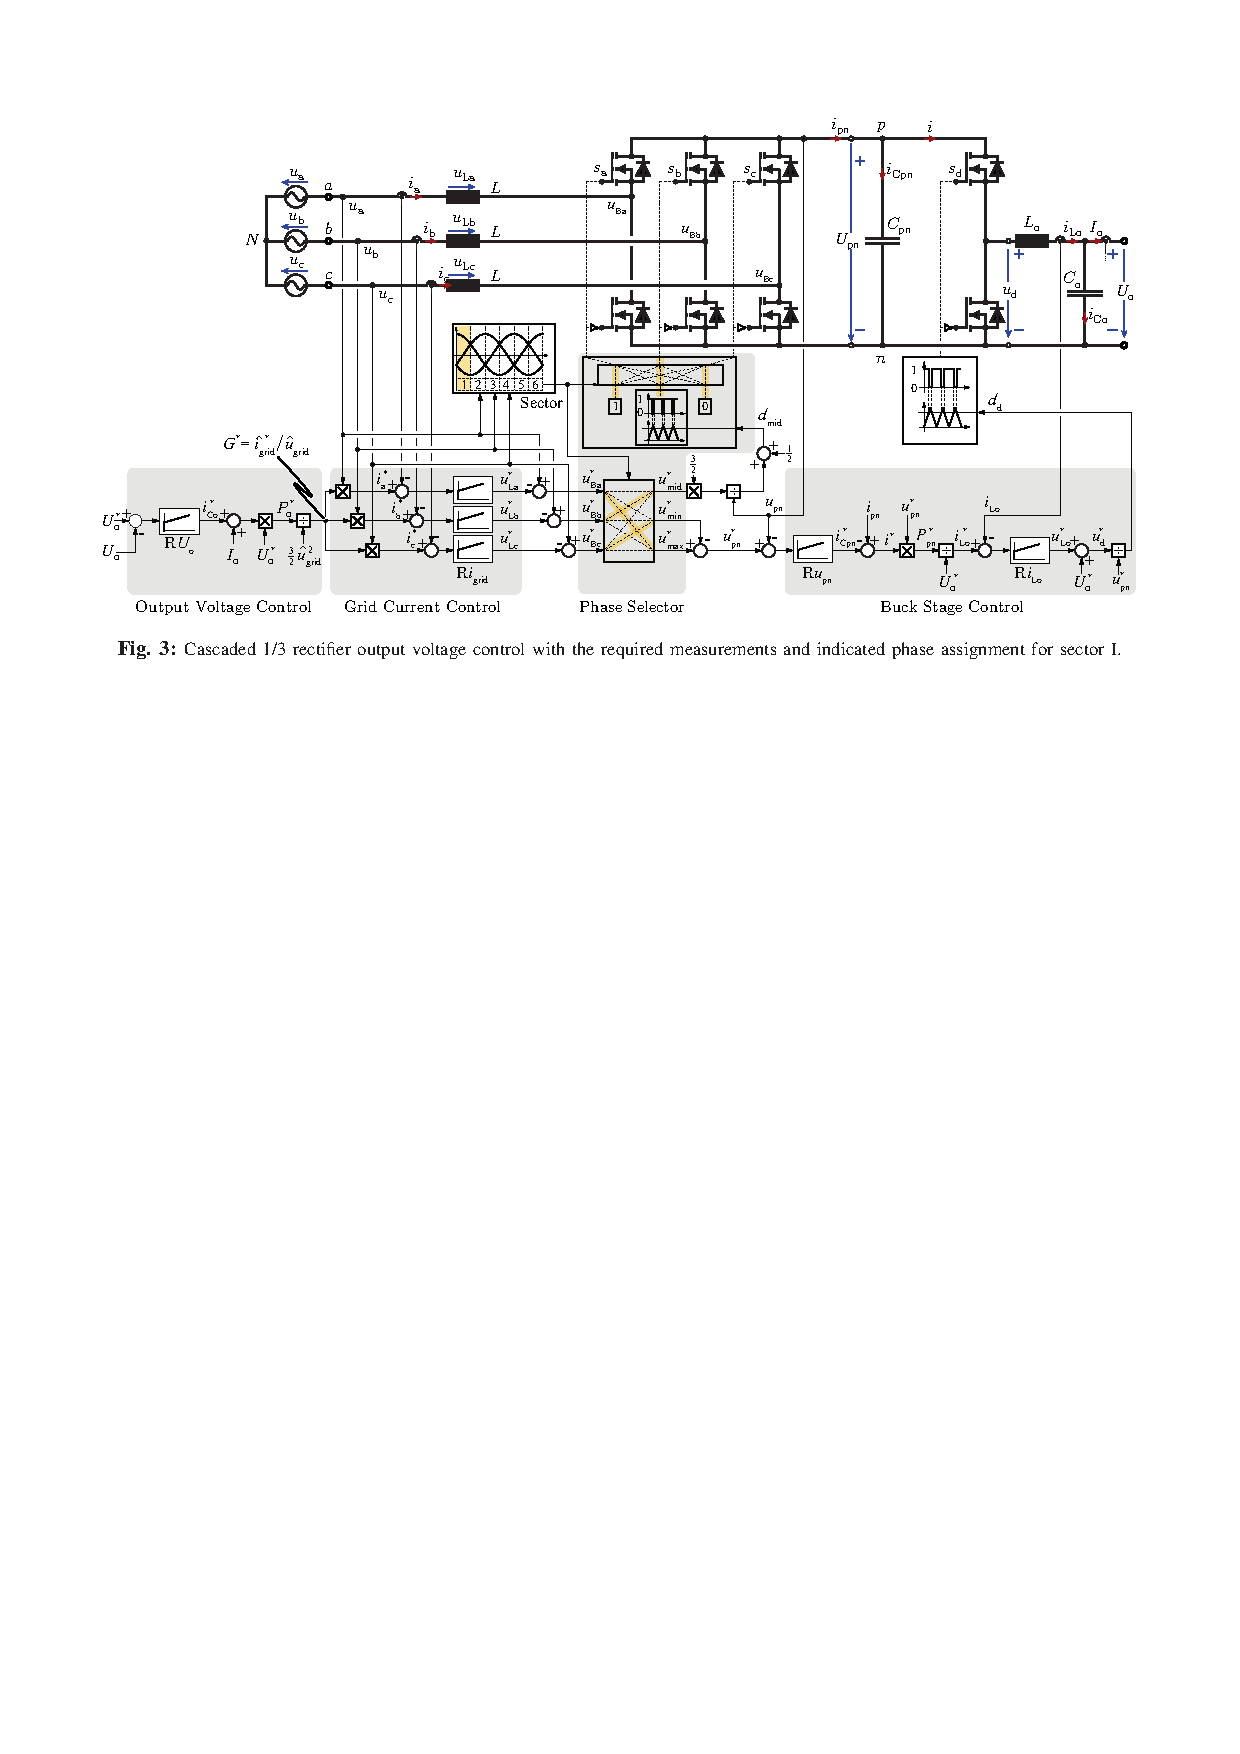
\includegraphics[width=0.65\linewidth]{content/Anhang/B6_Regelung}
	\caption{Regelungsstruktur des \gls{B6PFC} nach Menzi et Al. \cite{13PWMPFC}}
	\label{fig:b6regelung}
\end{figure}



\begin{table}
	\label{An:Entscheidungsmatrix}

\begin{tabular}{|c|c|c|c|c|c|}
	\hline
	Topologie & B6-Buck & Swiss & IAF & 6SwitchBuck & \% \\
	\hline
	L1 Netzinduktivität & 136 & 17,5 & 1 & 17,5 &\\
	\hline
	Gespeicherte Energie & 14,4 & 1,8 & 0,1 & 1,8 &\\
	\hline
	L2 DC Induktivität  & 136 & 136 & 136 & 136 &\\
	\hline
	Rippelstrom absolut & 88,5 & 88,5 & 88,5 & 88,5& \\
	\hline
	Gespeicherte Energie & 7,8 & 7,8 & 7,8 & 7,8 &\\
	\hline
	L3 IAF IVS Induktivität & - & - & 302,2 & - &\\
	\hline
	Gespeicherte Energie  & 0 & 0 & 2,6 & 0 &\\
	\hline
	Summe: & 22,2 & 9,6 & 10,6 & 9,6 &\\
	\hline
	\bfseries Induktivität normiert: & \bfseries 1 &\bfseries 0,43 &\bfseries 0,48 &\bfseries 0,43 & 50\\
	\hline
	C1 Netzkapazität & - & 50 & 50 & 50& \\
	\hline
	C2 am Elektrolyseur & 1 & 1 & 1 & 1 &\\
	\hline
	C3 DC Zwischenkreis & 25 & - & 50 & - &\\
	\hline
	\bfseries Kapazität normiert: &\bfseries 0,26 &\bfseries 0,5 &\bfseries 1 &\bfseries 0 &5\\
	\hline
	SiC 4mOhm & 0 & 0 & 2 & 0 &\\
	\hline
	SiC 2mOhm & 10 & 8 & 4 & 12 &\\
	\hline
	Vienna SiC 5mOhm & 0 & 6 & 6 & 0 &\\
	\hline
	\bfseries SiC normiert: &\bfseries 0,83 &\bfseries 0,87 &\bfseries 0,53 &\bfseries 1 &15\\
	\hline
	Vienna Diode & 0,0 & 6,0 & 6,0 & 0,0& \\
	\hline
	\bfseries Dioden normiert &\bfseries 0,0 & \bfseries1 &\bfseries 1 &\bfseries 0&5 \\
	\hline
	Treiberanzahl & 8 & 7 & 7 & 12 &\\
	\hline
	\bfseries Treiber normiert: &\bfseries 0,67 &\bfseries 0,58 &\bfseries 0,58 &\bfseries 1,00& 5\\
	\hline
	Schaltverluste 30 Grad & 567 & 215 & 503 & 303 &\\
	\hline
	Leitverluste 30 Grad & 254 & 1121 & 1311 & 543 &\\
	\hline
	Gewichtung 30 Grad & 75\% & 75\% & 75\% & 75\% &\\
	\hline
	Schaltverluste 0 Grad & 554 & 243 & 511 & 399& \\
	\hline
	Leitverluste 0 Grad & 326 & 781 & 748 & 722&\\
	\hline
	Gewichtung 0 Grad & 25\% & 25\% & 25\% & 25\%& \\
	\hline
	\bfseries Verluste normiert: &\bfseries 0,50 &\bfseries 0,75 &\bfseries 1,00 &\bfseries 0,55 &20\\
	\hline
	Gesamt &\bfseries 0,77 &\bfseries 0,6 &\bfseries 0,65 &\bfseries 0,55& \\
	\hline
\end{tabular}
\end{table}


